\documentclass{beamer}
\usetheme{Teema}

\usepackage{amsmath,amssymb,amsthm,enumerate,hyperref,mathdots}
\usepackage{multicol}
\usepackage[yyyymmdd]{datetime}\renewcommand{\dateseparator}{-}
\usepackage{ulem}
	\normalem
\usepackage[linguistics]{forest}
\newcommand{\tree}[1]{
	\begin{forest}
		for tree={
		inner sep=0pt,
		% where n children=0{font=\itshape}{},
	 %    calign=fixed edge angles,
	    parent anchor=south,
	  },
	  before typesetting nodes={% page 52: example (81)
	    where content={}{% shape=coordinate gives an error if used here but this is *almost* right - it just leaves a little, tiny gap
	      text width=.001pt,
	      inner sep=0pt,
	      before drawing tree={% here we make sure that the tiny gap disappears so only the size is not quite dimensionless
	        shape=coordinate,
	        typeset node,
	      },
	      for parent={
	        for children={
	          anchor=north,
	        }
	      }
	    }{}
	  }
	  #1
	\end{forest}
}

\title{Equivalence of generative systems and constraints:}
\subtitle{finite state automata and monadic second-order logic over strings}
\date{\today}
\author{\scshape{jacob louis hoover}}

\usepackage{gb4e}
\begin{document}
\maketitle
%--- Next Frame ---%

\begin{frame}{Outline}
\tableofcontents
\end{frame}

%%%%%%%%%%%%%%%%%%%%%%%%%%%%%%%%%%%%%%%%%%%%%%%%%%%%%%%%%%%
\section{Two basic approaches}%%%%%%%%%%%%%%%%%%%%%%%%%%%%%
%%%%%%%%%%%%%%%%%%%%%%%%%%%%%%%%%%%%%%%%%%%%%%%%%%%%%%%%%%%


%--- Next Frame ---%

\subsection{Minimalist Grammar - a generative system}
%--- Next Frame ---%

\begin{frame}
\begin{multicols}{2}
Given some lexical items:
\begin{itemize}
\item build :: =d d= v
\item rules :: n
\item trees :: n
\item these :: =n d
\item some  :: =n d
\item \emph{$\varnothing$} :: =n d
\end{itemize}
	\columnbreak
	\pause
	\tree{
		[v 
			[d 
				[{=n d\\these}] 
				[{n\\rules}]]
			[{d= v } 
				[{=d d= v\\build}]
				[d
					[{=n d\\some}]
					[{n\\trees}]]]]
	}
\end{multicols}

The rules are a formal system that describes a set of structures.
\end{frame}


%--- Next Frame ---%



% \subsection{CFG - a generative system}
%--- Next Frame ---%

% \begin{frame}
% \begin{multicols}{3}
% Context free rules:
% \begin{itemize}
% \item S $\to$ DP VP
% \item VP $\to$ V DP
% \item DP $\to$ D NP
% \item NP $\to$ N
% \item V $\to$ \emph{build}
% \item D $\to$ \emph{these}
% \item D $\to$ \emph{$\varnothing$}
% \item N $\to$ \emph{rules}
% \item N $\to$ \emph{trees}
% \end{itemize}
% 	\columnbreak
% 	\pause
% 	\tree{
% 		[S [DP [D [these]] [NP [N [rules]]]] [VP [V [build]] [DP [D [$\varnothing$]] [NP [N [trees]]]]]]
% 	}
% 	\columnbreak
% 	\pause
% 	\tree{
% 		[S [DP [D [$\varnothing$]] [NP [N [trees]]]] [VP [V [build]] [DP [D [$\varnothing$]] [NP [N [rules]]]]]]
% 	}
% \end{multicols}
% \end{frame}



%--- Next Frame ---%

% \subsection{X-bar theory - a generative system}


% \begin{frame}
% Phrase structure rules (for any lexical category X, X^0 = Head)
% \begin{itemize}
% \item 
% XP $\to$ specifier $\overline{\text{X}}$
% \item 
% $\overline{\text{X}}$ $\to$ X^0 (YP)^* = complement(s)
% \end{itemize}
% \pause 
% Builds a tree:
% \tree{[XP [specifier] [$\overline{\text{X}}$ [X^0 [head]] [complement(s)]]]}
% \end{frame}


\subsection{Binding theory - a system of constraints}%%%%%%%

%--- Next Frame ---%
\begin{frame}
	\begin{itemize}
	\item	\uline{Principle A}: An anaphor must be bound locally.
	\item	\uline{Principle B}: A pronoun must not be bound locally.
	\item	\uline{Principle C}: An R-expression must not be bound.
	\end{itemize}
	\pause
\begin{small}
\begin{multicols}{3}
\alert<3>{\tree{
	[S [it_1] [[described] [{the sentence}_1]]]
}}
\only<3>{Violates C!}
\columnbreak
\alert<3>{\tree{
	[S [{the sentence}_1] [[described] [it_1]]]
}}
\only<3>{Violates B!}
\columnbreak
\uncover<2->{\tree{
	[S [{the sentence}_1] [[described] [itself_1]]]
}
\tree{
	[S [it_1] [[described] [itself_1]]]
}
}
\end{multicols}\end{small}
\end{frame}

%--- Next Frame ---%
\begin{frame}
\uline{Principle A}: \emph{An anaphor must be bound by an element in argument position within its governing category.}

This is a logical statement about trees.

\pause

This can be formalized. 
E.g.:
\begin{align*}
	(\forall x,\forall X)	&[+\mathrm{anaphor}(x)\land \mathrm{GC}(X,x)]\to\\
					&(\exists y)[X(y)\land \mathrm{A\mbox{-}position}(y)\land \mathrm{c\mbox{-}command}(x,y) \land \mathrm{coindexed}(x,y)]]
\end{align*}
\pause

This is (more or less) from Jim Rogers translation of GB into logic.

I won't talk about this, but a similar, simpler version.
\end{frame}

\subsection{Both approaches}%%%%%%%%

%--- Next Frame ---%
%--- Next Frame ---%
\begin{frame}


Define a set of structures.

\pause
Linguistic theories are often formulated as a mix of both of these approaches.

\pause
\begin{enumerate}
\item Generative systems
	\begin{itemize}
	\item Phrase Structure Grammar
	\item Minimalism
	\item ...
	\end{itemize}
\item Constraint-based systems
	\begin{itemize}
	\item Government and Binding
	\item ...
	\end{itemize}
\end{enumerate}
\pause Are these equivalent? Can one be translated into the other?
\pause If yes... efficiently?
\end{frame}

%%%%%%%%%%%%%%%%%%%%%%%%%%%%%%%%%%%%%%%%%%%%%%%%%%%%%%%%%%%
\section{FSA and MSOL[$S$] over strings}%%%%%%%%%%%%%%%%%%%%%%%%
%%%%%%%%%%%%%%%%%%%%%%%%%%%%%%%%%%%%%%%%%%%%%%%%%%%%%%%%%%%

\subsection{Finite state automata}
%--- Next Frame ---%

\begin{frame}
A finite state automaton is a simple generative system.

\pause

A minimalist grammar where all lexical items are of the following form (having at most one selectional feature only on the right):

\begin{itemize}
\item a :: (=y) x
\end{itemize}

is a finite state automaton.

\end{frame}
%--- Next Frame ---%

\begin{frame}
\begin{multicols}{2}
For example, let $V= \{a,b\}$.

Take FSA $\mathcal A$:
\begin{center}
\begin{tikzpicture}[scale=0.2]
\tikzstyle{every node}+=[inner sep=0pt]
\draw [black] (28.6,-28.6) circle (3);
\draw (28.6,-28.6) node {q_0};
\draw [black] (28.6,-28.6) circle (2.4);
\draw [black] (41.9,-28.6) circle (3);
\draw (41.9,-28.6) node {q_1};
\draw [black] (27.277,-25.92) arc (234:-54:2.25);
\draw (28.6,-21.35) node [above] {$b$};
\fill [black] (29.92,-25.92) -- (30.8,-25.57) -- (29.99,-24.98);
\draw [black] (31.461,-27.709) arc (102.42208:77.57792:17.615);
\fill [black] (39.04,-27.71) -- (38.37,-27.05) -- (38.15,-28.03);
\draw (35.25,-26.8) node [above] {$a$};
\draw [black] (39.044,-29.506) arc (-77.35979:-102.64021:17.338);
\fill [black] (31.46,-29.51) -- (32.13,-30.17) -- (32.35,-29.19);
\draw (35.25,-30.43) node [below] {$a$};
\draw [black] (40.577,-25.92) arc (234:-54:2.25);
\draw (41.9,-21.35) node [above] {$b$};
\fill [black] (43.22,-25.92) -- (44.1,-25.57) -- (43.29,-24.98);
\draw [black] (23.3,-28.6) -- (25.6,-28.6);
\fill [black] (25.6,-28.6) -- (24.8,-28.1) -- (24.8,-29.1);
\end{tikzpicture}
\end{center}
\pause Accepts any string on $V^*$ with an even number of $a$s.  

\columnbreak

\pause

Grammar for this language:
\begin{itemize}
\item $a$ :: =q_1 q_0
\item $a$ :: =q_0 q_1
\item $b$ :: =q_0 q_0
\item $b$ :: =q_1 q_1
\item $\varepsilon$ :: q_0
\end{itemize}
\begin{small}
\pause
\tree{
	[q_0
	[{=q_1 q_0\\$a$}]
	[q_1
		[{=q_1 q_1\\$b$}]
		[q_1
		[{=q_0 q_1\\$a$}]
		[{q_0\\$\varepsilon$}]]]]
}\end{small}
\end{multicols}
\end{frame}
%--- Next Frame ---%

\begin{frame}
The class of strings accepted by finite state automata can also be descibed in terms of constraints. 
\begin{itemize}
\item ``there are an even number of $a$'s in the string''
\end{itemize}

\pause

\begin{block}{Question:}
given a language (a set of strings) generated by a FSA, what kind of constraints are needed to define it?
\end{block}
\pause
\begin{block}{Answer:}
If a language can be generated by a FSA, it can be defined using constraints written in \underline{monadic second-order logic} (with a successor).
\end{block}

\end{frame}
%--- Next Frame ---%



\begin{frame}
In fact, this generative system (any FSA you can build) and this system of constraints (anything you can write in the logic MSOL[$S$]) are equivalent in expressive power: they both describe the same class of languages.

\pause

First, to formalize:
\begin{itemize}
\item FSA
\item Strings as models
\item MSOL
\end{itemize}
\end{frame}


%--- Next Frame ---%

\begin{frame}
A finite state automaton $\mathcal A=(V,Q,q_0,F,\Delta)$, consisting of
\begin{itemize}
\item the vocabulary $V$
\item $Q$ is a finite set of states $q_0,q_1,\dots,q_k$
	\begin{itemize}
	\item $q_0\in Q$ is the \emph{initial} state 
	\item $F\subseteq Q$ is set of \emph{final} (or \emph{accepting}) states
	\end{itemize}
\item $\Delta\subseteq Q\times V\times Q$ is the \emph{transition relation} 
\end{itemize}
\pause
A string $\sigma=a_0\dots a_{n-1}$ is \underline{accepted} by $\mathcal A$ if there is a successful run of $\mathcal A$ on $\sigma$, that is, a sequence $\rho=\rho_0\dots\rho_n$ of states, such that $\rho_0=q_0$, $\rho_n\in F$, and $(\rho_i,a_i,\rho_{i+1})\in \Delta$ for $i<n$.
\begin{center}
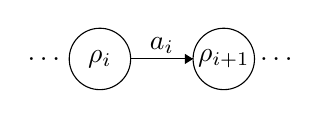
\begin{tikzpicture}[scale=0.13]
\tikzstyle{every node}+=[inner sep=0pt]
\draw [black] (27.4,-27.8) circle (3);
\draw (27.4,-27.8) node {$\rho_i$};
\draw [black] (39.5,-27.8) circle (3);
\draw (39.5,-27.8) node {$\rho_{i+1}$};
\draw [black] (30.4,-27.8) -- (36.5,-27.8);
\fill [black] (36.5,-27.8) -- (35.7,-27.3) -- (35.7,-28.3);
\draw (33.45,-27.3) node [above] {$a_i$};
\draw (24,-27.8) node [left] {$\dots$};
\draw (43,-27.8) node [right] {$\dots$};
\end{tikzpicture}
\end{center}
A language is accepted by $\mathcal A$ if all its strings are accepted.
\end{frame}

%--- Next Frame ---%
\subsection{Strings as models}
\begin{frame}
Let $V$ be a finite vocabulary and $\sigma = a_0\dots a_{n-1}$ be a string over $V$.  In order to interpret logical statements about this string, create a \emph{string model} of $\sigma$: 
\begin{equation}
\underline{\sigma} = (\mathrm{pos}(\sigma), S^\sigma, (Q^\sigma_a)_{a\in V})
\end{equation}
Where $\mathrm{pos(\sigma)}$ is $\{0,1,\dots,n-1\}$, the set of word positions in the string , $S^\sigma$ is the natural successor relation defined on these integers, and $Q_a^\sigma$ is a unary predicates collecting for $a\in V$ the positions in $\mathrm{pos(\sigma)}$ where $a$ occurs.
\pause

E.g. 
\begin{equation*}
\underline{bab} = (\{0,1,2\}, S^{bab}, Q^{bab}_a =\{1\}, Q^{bab}_b = \{0,2\})
\end{equation*}
\end{frame}

%--- Next Frame ---%
\subsection{Strings and logic}
\begin{frame}
Given string models over $V$, statements about the strings can be formalized in logic.


\only<1>{\textbf{First-order logic:}}
\only<2>{\textbf{Monadic second-order logic:}}
\begin{itemize}
\item variables
\begin{itemize}
	\item $x,y,x_i,\dots$		\hfill(range over positions in the string models)
	\item<2> $X,Y,X_i,\dots$	\hfill(range over sets of positions)
\end{itemize}
\item atomic formulæ:
	\begin{itemize}
	\item $x=y$					\hfill(equality)
	\item $S(x,y)$ 				\hfill(the successor of $x$ is $y$)
	\item $Q_a(x)$, $a\in V$	\hfill(position $x$ has label $a$)
	\item<2> $X(x)$ 			\hfill(set $X$ contains element $x$)
	\end{itemize}
\item connectives: $\land,\lor,\lnot,\rightarrow,\leftrightarrow$ and quantifiers: $\exists, \forall$

\end{itemize}


\end{frame}
%--- Next Frame ---%

\begin{frame}

For example: take the first-order sentence $\phi = \exists x. [Q_a(x)\land \lnot \exists y . S(x,y)]$\hfill``the string ends in $a$''
\pause

To evaluate this on string $ba$: take the model $\uline{ba}$, and see whether $\exists x. [Q^{ba}_a(x)\land \lnot \exists y . S^{ba}(x,y)]$ is true.  \pause \checkmark

\pause 
So, we say $\uline{ba}\models\phi$: $ba$ \emph{models} $\phi$.
\end{frame}
%--- Next Frame ---%


\begin{frame}
\begin{center}
\begin{tikzpicture}[scale=0.1]
\tikzstyle{every node}+=[inner sep=0pt]
\draw [black] (28.6,-28.6) circle (3);
\draw (28.6,-28.6) node {q_0};
\draw [black] (28.6,-28.6) circle (2.4);
\draw [black] (41.9,-28.6) circle (3);
\draw (41.9,-28.6) node {q_1};
\draw [black] (27.277,-25.92) arc (234:-54:2.25);
\draw (28.6,-21.35) node [above] {$b$};
\fill [black] (29.92,-25.92) -- (30.8,-25.57) -- (29.99,-24.98);
\draw [black] (31.461,-27.709) arc (102.42208:77.57792:17.615);
\fill [black] (39.04,-27.71) -- (38.37,-27.05) -- (38.15,-28.03);
\draw (35.25,-26.8) node [above] {$a$};
\draw [black] (39.044,-29.506) arc (-77.35979:-102.64021:17.338);
\fill [black] (31.46,-29.51) -- (32.13,-30.17) -- (32.35,-29.19);
\draw (35.25,-30.43) node [below] {$a$};
\draw [black] (40.577,-25.92) arc (234:-54:2.25);
\draw (41.9,-21.35) node [above] {$b$};
\fill [black] (43.22,-25.92) -- (44.1,-25.57) -- (43.29,-24.98);
\draw [black] (23.3,-28.6) -- (25.6,-28.6);
\fill [black] (25.6,-28.6) -- (24.8,-28.1) -- (24.8,-29.1);
\end{tikzpicture}
\end{center}
\pause
\vspace*{-10pt}
To capture the same language with a MSOL constraint:

\pause
\begin{small}
First, define the ordering ``$<$'':
\pause
$x<y:=\hfill \lnot (x=y) \land \forall X[X(x) \land \forall z\forall w (X(z)\land S(z,w)\to X(w))\to X(y)]$
\pause
and define some shorthand:

$\phi(\mathrm{first}_a):=\hfill  \exists x.\phi(x)\land Q_a(x)\land(\lnot\exists z. z<x \land Q_a(z))$ 

$\phi(\mathrm{last}_a):=\hfill  \exists x.\phi(x)\land Q_a(x)\land(\lnot\exists z. x<z \land Q_a(z))$ 

$\mathrm{next}_a(x,y):=\hfill  Q_a(x)\land Q_a(y) \land (\lnot \exists z. x<z\land z<y \land Q_a(z) ) $
\pause
\end{small}
\begin{align*}
\forall x. &Q_a(x)\to \exists X.X(\mathrm{first}_a) \\
& \land \forall y \forall z .
	[\mathrm{next}_a(y,z) \to (X(y)\leftrightarrow\lnot X(z))]\\
&\land\lnot X(\mathrm{last}_a)
\end{align*}
\end{frame}

\subsection{The equivalence of FSAs and MSOL[$S$]}
\begin{frame}
\begin{block}{Theorem}
A language $L$ of finite-length strings is can be generated by a FSA
iff 
$L$ is definable in MSOL[$S$].
\end{block}
\pause

The proof consists of showing that

$(\rightarrow)$ given an automaton, we can write a formula, and 

$(\leftarrow)$ given a formula, we can construct an automaton.

\end{frame}

\subsubsection{proof ($\rightarrow$)}
\begin{frame}
Given automaton $\mathcal{A}=(V,Q,q_0,F,\Delta)$, write $\phi_{\mathcal{A}}$, a MSOL[$S$]-sentence (a formula with no free variables) such that $\uline{\sigma}\models\phi_{\mathcal{A}}$ for any string $\sigma$ that is accepted by $\mathcal{A}$.

\pause 
That is, $\phi_{\mathcal{A}}$ must express in $\uline{\sigma}$ the existence of an accepting run of $\mathcal A$ on $\sigma$. 

\pause
\textbf{Strategy:} Associate a set variable $X_i$ with each state $q_i$ in $\mathcal A$.  This set variable denotes the positions on the string when $\mathcal A$ assumes state $q_i$. 
\end{frame}

\begin{frame}
\only<1-4>{if $\mathcal{A}$ has $k$ states, we can use set variables $X_0,\dots,X$ to describe successful runs:
}
\only<5->{$\exists X_0,\dots,\exists X_k \Big[$}
\begin{itemize}
\item \only<1-5>{the $X_i$'s are pairwise disjoint sets over the positions (at any position in the string, the automaton is in exactly one state)} 
	\only<6->{$\bigwedge_{i\neq j}\forall x \lnot (X_i(x)\land X_j(x))$}
\item \only<2-6>{at the first position, the automaton is in initial state $q_0$}
	\only<7->{$\forall x (\lnot \exists y  S(y,x)\to X_0(x))$}
\item \only<3-7>{for any pair of successive positions in the string $x, y$, there is a valid transition given by the states at positions $x$ and $y$, and the label at position $x$}
	\only<8->{$\forall x \forall y  (S(x,y)\to \bigvee_{(q_i,a,q_j)\in\Delta} X_i(x)\land Q_a(x)\land X_j(y))$}
\item \only<4-8>{at the final position there is a valid transition into an accepting state}
	\only<9->{$\forall x (\lnot \exists y  S(x,y) \to \bigvee_{(q_i,a,q_j)\in \Delta, q_j\in F} X_i(x) \land Q_a(x) )\Big]$}
\end{itemize}
\only<10->{The form of this sentence: automata normal form.}

\end{frame}

\begin{frame}
$\mathcal A$ accepts/generates a string $\sigma$ iff 
\begin{align*}
 \uline{\sigma} \models \exists X_0 \dots \exists X_k\quad & \Big[\bigwedge_{i\neq j}\forall x \lnot (X_i(x)\land X_j(x))\\
 &\land \forall x (\lnot \exists y  S(y,x)\to X_0(x))\\
 &\land \forall x \forall y  (S(x,y)\to \bigvee_{(q_i,a,q_j)\in\Delta} X_i(x)\land Q_a(x)\land X_j(y)) \\
 &\land \forall x (\lnot \exists y  S(x,y) \to \bigvee_{(q_i,a,q_j)\in \Delta, q_j\in F} X_i(x) \land Q_a(x) )\Big]
\end{align*} 
\end{frame}

\subsubsection{proof ($\leftarrow$)}
\begin{frame}
In the other direction, show that given a formula $\phi$ of MSOL[$S$], we can construct an FSA $\mathcal{A}_\phi$, such that for any string which models the formula $\underline{\sigma}\models\phi$, this string is accepted by $\mathcal{A}_\phi$.

\pause

\textbf{Strategy:} A proof by induction on formulas. Show that for every atomic formula, there is a simple FSA that recognizes precisely the set of strings defined by that atomic formula.  

For the inductive step show that this property is closed under connectives and quantification.

\end{frame}

\begin{frame}
Work with the expressively equivalent (but syntactically simpler) MSOL$_0$[$S$]:
\begin{itemize}
\item 
has only set variables (first order variables $x$ are converted to singleton set variables $X$). 
\item 
connectives $\lnot$ and $\lor$, and quantification $\exists$. 
\end{itemize}

This means the proof must just
\begin{itemize}
\item construct an FSA that is equivalent to each atomic formula of MSOL$_0$[$S$]
\item show that the class of recognizable languages is closed under complement and union and projection
\end{itemize}
\end{frame}

\subsection{And so forth}
\begin{frame}
Consequences and corollaries:
\begin{itemize}
\item Any MSOL[$S$] formula can be written as one in `automata normal form'.
\pause 
\item General translation of logic to automata: hard.  \pause In general, it has been shown that time-complexity of \emph{any algorithm} converting MSOL[$S$] $\to$ automata \emph{cannot be bounded by any elementary function} (there is an unbounded family of formulæ the corresponding automaton's number of states grows with length of formula like $2\uparrow\uparrow n = \underbrace{2^{2^{\iddots^{2}}}}_{n}$. That's a hefty lower bound.
\end{itemize}
\end{frame}


\subsection{And so on}
\begin{frame}
So, MSOL is a nice way to describe languages that can be accepted by FSAs.
\pause Translating in general is hard, but... most things that can be said in logic are not things we want to say.
\end{frame}
\begin{frame}{\ }


\begin{center}
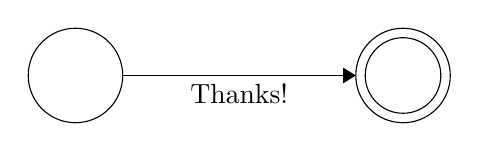
\begin{tikzpicture}[scale=0.2]
\tikzstyle{every node}+=[inner sep=0pt]
\draw [black] (34.8,-27.9) circle (3);
\draw [black] (34.8,-27.9) circle (2.4);
\draw [black] (14,-27.9) circle (3);
\draw [black] (17,-27.9) -- (31.8,-27.9);
\fill [black] (31.8,-27.9) -- (31,-27.4) -- (31,-28.4);
\draw (24.4,-28.4) node [below] {Thanks!};
\end{tikzpicture}
\end{center}
\end{frame}
\end{document}
